\documentclass[aspectratio=169]{../latex_main/tntbeamer}  % you can pass all options of the beamer class, e.g., 'handout' or 'aspectratio=43'
\usepackage{dsfont}
\usepackage{bm}
\usepackage[english]{babel}
\usepackage[T1]{fontenc}
%\usepackage[utf8]{inputenc}
\usepackage{graphicx}
\graphicspath{ {./figures/} }
\usepackage{algorithm}
\usepackage[ruled,vlined,algo2e,linesnumbered]{algorithm2e}
\usepackage{hyperref}
\usepackage{booktabs}
\usepackage{mathtools}

\usepackage{amsmath,amssymb}

\DeclareMathOperator*{\argmax}{arg\,max}
\DeclareMathOperator*{\argmin}{arg\,min}

\usepackage{amsbsy}
\newcommand{\vect}[1]{\bm{#1}}
%\newcommand{\vect}[1]{\boldsymbol{#1}}

\usepackage{pgfplots}
\pgfplotsset{compat=1.16}
\usepackage{tikz}
\usetikzlibrary{trees} 
\usetikzlibrary{shapes.geometric}
\usetikzlibrary{positioning,shapes,shadows,arrows,calc,mindmap}
\usetikzlibrary{positioning,fadings,through}
\usetikzlibrary{decorations.pathreplacing}
\usetikzlibrary{intersections}
\pgfdeclarelayer{background}
\pgfdeclarelayer{foreground}
\pgfsetlayers{background,main,foreground}
\tikzstyle{activity}=[rectangle, draw=black, rounded corners, text centered, text width=8em]
\tikzstyle{data}=[rectangle, draw=black, text centered, text width=8em]
\tikzstyle{myarrow}=[->, thick, draw=black]

% Define the layers to draw the diagram
\pgfdeclarelayer{background}
\pgfdeclarelayer{foreground}
\pgfsetlayers{background,main,foreground}

% Requires XeLaTeX or LuaLaTeX
%\usepackage{unicode-math}

\usepackage{fontspec}
%\setsansfont{Arial}
\setsansfont{RotisSansSerifStd}[ 
Path=../latex_main/fonts/,
Extension = .otf,
UprightFont = *-Regular,  % or *-Light
BoldFont = *-ExtraBold,  % or *-Bold
ItalicFont = *-Italic
]
\setmonofont{Cascadia Mono}[
Scale=0.8
]

% scale factor adapted; mathrm font added (Benjamin Spitschan @TNT, 2021-06-01)
%\setmathfont[Scale=1.05]{Libertinus Math}
%\setmathrm[Scale=1.05]{Libertinus Math}

% other available math fonts are (not exhaustive)
% Latin Modern Math
% XITS Math
% Libertinus Math
% Asana Math
% Fira Math
% TeX Gyre Pagella Math
% TeX Gyre Bonum Math
% TeX Gyre Schola Math
% TeX Gyre Termes Math

% Literature References
\newcommand{\lit}[2]{\href{#2}{\footnotesize\color{black!60}[#1]}}

%%% Beamer Customization
%----------------------------------------------------------------------
% (Don't) Show sections in frame header. Options: 'sections', 'sections light', empty
\setbeamertemplate{headline}{empty}

% Add header logo for normal frames
\setheaderimage{
	% 
\includegraphics[height=\logoheight]{figures/TNT_darkv4.pdf}
	
\includegraphics[height=\logoheight]{../latex_main/figures/luh_logo_rgb_0_80_155.pdf}
	% 
\includegraphics[height=\logoheight]{figures/logo_tntluh.pdf}
}

% Header logo for title page
\settitleheaderimage{
	% 
\includegraphics[height=\logoheight]{figures/TNT_darkv4.pdf}
	
\includegraphics[height=\logoheight]{../latex_main/figures/luh_logo_rgb_0_80_155.pdf}
	% 
\includegraphics[height=\logoheight]{figures/logo_tntluh.pdf}
}

% Title page: tntdefault 
\setbeamertemplate{title page}[tntdefault]  % or luhstyle
% Add optional title image here
%\addtitlepageimagedefault{
\includegraphics[width=0.65\textwidth]{figures/luh_default_presentation_title_image.jpg}}

% Title page: luhstyle
% \setbeamertemplate{title page}[luhstyle]
% % Add optional title image here
% \addtitlepageimage{
\includegraphics[width=0.75\textwidth]{figures/luh_default_presentation_title_image.jpg}}

\author[Abedjan \& Lindauer]{Ziawasch Abedjan \& Marius Lindauer\\[1em]
	
\includegraphics[height=\logoheight]{../latex_main/figures/luh_logo_rgb_0_80_155.pdf}\qquad
	
\includegraphics[height=\logoheight]{../latex_main/figures/DBIS_Kurzlogo.png}\qquad

\includegraphics[height=\logoheight]{../latex_main/figures/TNT_darkv4}\qquad

\includegraphics[height=\logoheight]{../latex_main/figures/L3S.jpg}	}
\date{Summer Term 2022; \hspace{0.5em} {
\includegraphics[height=1.5em]{../latex_main/figures/Cc-by-nc-sa_icon.svg.png}}; based on \href{https://ds100.org/fa21/}{[DS100]}
}


%%% Custom Packages
%----------------------------------------------------------------------
% Create dummy content
\usepackage{blindtext}

% Adds a frame with the current page layout. Just call \layout inside of a frame.
\usepackage{layout}


%%% Macros
%\renewcommand{\vec}[1]{\mathbf{#1}}
% \usepackage{bm}
%\let\vecb\bm

\title[Regression]{DS: Ordinary Least Squares}
\subtitle{Problem statement}

\graphicspath{ {./figure_ols/} }
%\institute{}


\begin{document}
	
	\maketitle
	\begin{frame}{Vector norms}
	    \begin{itemize}
	        \item The norm of a vector is some measure of that vector’s size.
	        \item  The two norms we need to know (for now) are the L1 and L2 norms.
	        \begin{itemize}
	            \item We will mainly focus on $L_2$ today.
	            %\item $L_1$ will appear a few lectures from now.
	        \end{itemize}
	    \end{itemize}
	    \begin{columns}
	        \begin{column}{.4\textwidth}
	        Consider the vector:

	                \vect{x} = $\left[\begin{array}{c}
	          x_1\\
	          x_2 \\
	          x_3 \\
	          \vdots\\
	          x_n
	    \end{array}\right]$
	        \end{column}
	        
	        
	        
	         \begin{column}{.5\textwidth}
	                $L_2$ vector norm:
	                \begin{equation*}
	                    ||\vect{x}||_2 = \sqrt{x_1^2 + x_2^2 + x_3^2 + ... + x_n^2} = \sqrt{\sum\limits_{i=1}^nx_i^2}
	                \end{equation*}
	                $L_1$ vector norm:
	                \begin{equation*}
	                    ||\vect{x}||_1 = |x_1| + |x_2| + |x_3| + ... +|x_n| = \sum\limits_{i=1}^n|x_i| 
	                \end{equation*}
	        \end{column}
	    \end{columns}
	\end{frame}
	
	
	\begin{frame}{$L_2$ vector norm}
	    \begin{itemize}
	        \item The $L_2$ vector norm can be thought of as the “length” of a vector.
	        \begin{itemize}
	            \item It is a generalization of the Pythagorean theorem into n dimensions.
	            \begin{equation*}
	                    ||\vect{x}||_2 = \sqrt{x_1^2 + x_2^2 + x_3^2 + ... + x_n^2} = \sqrt{\sum\limits_{i=1}^nx_i^2}
	             \end{equation*}
	        \end{itemize}
	        \item  The “distance” between two vectors is the L2 norm of their difference.
	        \begin{itemize}
	            \item For instance, if $\vect{a}$ and $\vect{b}$ are two vectors of the same length, then their distance is
                \begin{equation*}
                    ||\vect{a}-\vect{b}||_2
                \end{equation*}
	        \end{itemize}
	        \item Note, the square of the L2 norm of a vector is the sum of the squares of the vector’s elements:
	    \end{itemize}
	    \begin{equation*}
                    ||\vect{x}||_2^2 = \sum\limits_{i=1}^nx_i^2
        \end{equation*}
	\end{frame}
	
	
	
	\begin{frame}{Residuals}
	    \begin{columns}
	        \begin{column}{.4\textwidth}
	        	Residuals are defined as being the difference between an actual and predicted value, in the regression context.
	        	\begin{itemize}
	        	    \item We use the letter $e$ to denote residuals. The $i$-th residual is\\
	        	    $e_i = y_i - \hat{y_i}$
	        	    \item The MSE of a model is equal to the mean of the squares of its residuals:
	        	\end{itemize}
	        	\begin{equation*}
	        	    MSE = \frac{1}{n}\sum\limits_{i=1}^ne_i^2
	        	\end{equation*}
	        \end{column}

	         \begin{column}{.6\textwidth}

                        \vspace{-3em}
	                    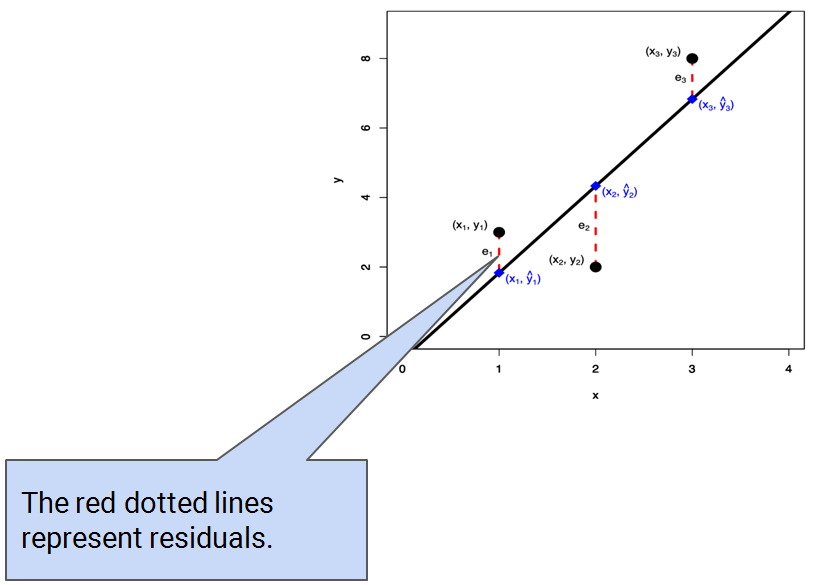
\includegraphics[scale=.44]{Bild4}

	        \end{column}
	    \end{columns}
	\end{frame}
	
	\begin{frame}{Residual vector}
	    We can stack all $n$ residuals into a vector, called the residual vector, $\vect{e}$:
        \begin{equation*}
            \vect{e} = \vect{Y} - \hat{\vect{Y}}  =\left[\begin{array}{c}
                 y_1 - \hat{y_1}\\
                 y_2 - \hat{y_2}\\
                 \vdots\\
                 y_n - \hat{y_n}\\
            \end{array}\right]
        \end{equation*}
        The residual vector is the “difference” between the two vectors containing our true $y$ values and predicted $y$ values. 

	\end{frame}
	
	
	\begin{frame}{Mean squared error, again}
	    We are choosing our loss to be squared loss. This means, the average loss across our dataset is mean squared error.
        \begin{equation*}
            R(\vect{\theta} ) = \frac{1}{n}\sum_{i=1}^n(y_i - \hat{y_i})^2 = \frac{1}{n}\sum_{i=1}^n(y_i - \vect{X}_i^\intercal\vect{\theta})^2
        \end{equation*}
        We can write this in terms of the norm of the residual vector!
        \begin{equation*}
            R(\theta ) = \frac{1}{n}||\vect{Y} - \hat{\vect{Y}}||_2^2 = \frac{1}{n}||\vect{Y} - \vect{X}\vect{\theta}||_2^2
        \end{equation*}
       % $\vect{X}$ is the residual vector
	\end{frame}
	
	
	
	\begin{frame}{Optimization procedure}
	    As we did before, we note that the value of $\vect{\theta}$ that minimizes  $\frac{1}{n}||\vect{Y} - \vect{X}\vect{\theta}||_2^2$                     is the same value that minimizes

        \begin{equation*}
            R(\vect{\theta} ) = ||\vect{Y} - \vect{X}\vect{\theta}||_2^2
        \end{equation*}
        Therefore, our goal is to find the value of     $\vect{\theta}$   that minimizes the squared $L_2$ norm of the residual vector. In other words, we want the “distance” between   $\vect{Y}$   and    $\hat{\vect{Y}}$    to be minimized\\
        \bigskip
        There are two ways we can determine the optimal $\hat{\vect{\theta}}$     here.
        \begin{itemize}
            \item Using calculus, like we’ve done earlier.
            \item Using a geometric argument. This is what we’ll do next.
        \end{itemize}
	\end{frame}
\end{document}